\qrchapter{https://forgottenpillar.com/rsc/en-fp-chapter8}{The constructive criticism}


\qrchapter{https://forgottenpillar.com/rsc/en-fp-chapter8}{La critique constructive}


The first point of the \emcap{Fundamental Principles} answers the questions: who is God, what is His personality, and how do we understand His presence?


Le premier point des \emcap{Principes Fondamentaux} répond aux questions : qui est Dieu, quelle est Sa personnalité, et comment comprenons-nous Sa présence ?


\others{I. That there is \textbf{one God}, \textbf{a personal, spiritual }\textbf{\underline{being}}, \textbf{the creator of all things}, omnipotent, omniscient, and eternal; infinite in wisdom, holiness, justice, goodness, truth, and mercy; unchangeable, and \textbf{everywhere present by his representative, the Holy Spirit}. Ps. 139:7.}[FP1889 147.2; 1889][https://egwwritings.org/read?panels=p931.6]


\others{I. Qu'il y a \textbf{un seul Dieu}, \textbf{un \underline{être} personnel et spirituel}, \textbf{le créateur de toutes choses}, omnipotent, omniscient et éternel ; infini en sagesse, sainteté, justice, bonté, vérité et miséricorde ; immuable, et \textbf{présent partout par son représentant, le Saint-Esprit}. Ps. 139:7.}[FP1889 147.2; 1889][https://egwwritings.org/read?panels=p931.6]


The one God, the Creator, is identified as the Father, because the second point of the \emcap{Fundamental Principles} states that Jesus Christ, the Son of the Eternal Father, is the one by whom God created all things\footnote{\href{https://egwwritings.org/?ref=en_FP1889.147.3&para=931.7}{FP1889 147.3; 1889}}. The \emcap{personality of God} is expressed in the term “\textit{personal spiritual being}”. We will soon see that this term denotes that the Father has a material body, a physical manifestation. Thus, in His personality, He is present only where He dwells physically. But, His presence is not constrained to His personality because He is \others{everywhere present by his representative, the Holy Spirit}. During our past history, this understanding and reasoning of the \emcap{personality of God}, as expressed in the first point of the \emcap{Fundamental Principles}, received constructive criticism; by “constructive criticism” we refer to the criticism supported by the Bible.


Le seul Dieu, le Créateur, est identifié comme le Père, car le deuxième point des \emcap{Principes Fondamentaux} déclare que Jésus-Christ, le Fils du Père Éternel, est celui par qui Dieu a créé toutes choses\footnote{\href{https://egwwritings.org/?ref=en_FP1889.147.3&para=931.7}{FP1889 147.3; 1889}}. La \emcap{personnalité de Dieu} est exprimée dans le terme “\textit{être personnel et spirituel}”. Nous verrons bientôt que ce terme indique que le Père a un corps matériel, une manifestation physique. Ainsi, dans Sa personnalité, Il n'est présent que là où Il demeure physiquement. Mais Sa présence n'est pas limitée à Sa personnalité car Il est \others{présent partout par son représentant, le Saint-Esprit}. Au cours de notre histoire passée, cette compréhension et ce raisonnement de la \emcap{personnalité de Dieu}, tels qu'exprimés dans le premier point des \emcap{Principes Fondamentaux}, ont reçu des critiques constructives ; par “critiques constructives”, nous faisons référence aux critiques soutenues par la Bible.


We now present to you the following citations, some constructive criticism, from a prominent trinitarian brother in the Seventh-day Adventist world. Interestingly, he had acknowledged the authority of the \emcap{Fundamental Principles}, yet simultaneously believed in the Trinity doctrine. We find this document a very important element in the change of our beliefs from the fundamental principles to current Seventh-day Adventist Trinitarian belief.


Nous vous présentons maintenant les citations suivantes, quelques critiques constructives, d'un frère trinitaire éminent dans le monde adventiste du septième jour. Il est intéressant de noter qu'il avait reconnu l'autorité des \emcap{Principes Fondamentaux}, tout en croyant simultanément à la doctrine de la Trinité. Nous considérons ce document comme un élément très important dans le changement de nos croyances, passant des principes fondamentaux à la croyance trinitaire adventiste actuelle.


This prominent brother was met with the question, “\textit{Do you not believe in a personal, definite God?}”:


Ce frère éminent a été confronté à la question : “\textit{Ne croyez-vous pas en un Dieu personnel et défini ?}” :


\others{\textbf{Most certainly. An infinite, divine, personal being is essential religion}. Worship requires someone to love, to obey, to trust. \textbf{Belief in a personal God is the very core of the Christian religion}. The conception of God as the All-Energy, the infinite Power, an all-pervading Presence, is too vast for the human mind to grasp; there must be something more \textbf{tangible}, more \textbf{\underline{restricted}}, upon which to center the mind in worship. \textbf{It is for this reason that Christ came to us in the image of God's }\textbf{\underline{personality}}\textbf{, the second Adam, to show us by his life of love and self-sacrifice the character and }\textbf{\underline{the personality of God}}. We can approach God only through Christ.}


\others{\textbf{Très certainement. Un être personnel, divin et infini est essentiel à la religion}. L'adoration nécessite quelqu'un à aimer, à obéir, à qui faire confiance. \textbf{La croyance en un Dieu personnel est le cœur même de la religion chrétienne}. La conception de Dieu comme l'Énergie-Totale, la Puissance infinie, une Présence omniprésente, est trop vaste pour que l'esprit humain puisse la saisir ; il doit y avoir quelque chose de plus \textbf{tangible}, plus \textbf{\underline{restreint}}, sur quoi centrer l'esprit dans l'adoration. \textbf{C'est pour cette raison que Christ est venu à nous à l'image de la }\textbf{\underline{personnalité}}\textbf{ de Dieu, le second Adam, pour nous montrer par sa vie d'amour et d'abnégation le caractère et }\textbf{\underline{la personnalité de Dieu}}. Nous ne pouvons approcher Dieu que par Christ.}


\othersnogap{‘Who being the brightness of his glory, and \textbf{the express image of his person}, and upholding all things by the word of his power, when he had by himself purged our sins, sat down on the right hand of the Majesty on high.’}


\othersnogap{‘Qui, étant le rayonnement de sa gloire et \textbf{l'empreinte de sa personne}, et soutenant toutes choses par la parole de sa puissance, après avoir fait par lui-même la purification de nos péchés, s'est assis à la droite de la Majesté divine dans les lieux très hauts.’}


\othersnogap{‘Who being the effulgence of his glory, and the impress of his substance, and upholding all things by the word of his power.’}


\othersnogap{‘Qui, étant le rayonnement de sa gloire, et l'empreinte de sa substance, et soutenant toutes choses par la parole de sa puissance.’}


\othersnogap{The apostle says, ‘But we all, with open face \textbf{beholding as in a glass} the glory of the Lord, are changed into the same image from glory to glory, even as by the Spirit of the Lord.’ 2 Cor. 3: 18. How apt and beautiful is this figure!... So, \textbf{in beholding Christ} in his miracles, his temptations, his exhortations, his life of self-abnegation, his ‘going about doing good,’ \textbf{we may behold the personality and power of God}. And what a great hope there is for us in the fact that \textbf{in Christ we find qualities not strange and foreign to humanity}, but kindred mental and moral characteristics; so that we are able to see and grasp an actual, rather than merely a theological or abstract or figurative truth, in the declaration of the apostle, ‘Now are we the sons of God.’ 1 John 3:2.}


\othersnogap{L'apôtre dit : ‘Nous tous qui, \textbf{le visage découvert, contemplons comme dans un miroir} la gloire du Seigneur, nous sommes transformés en la même image, de gloire en gloire, comme par l'Esprit du Seigneur.’ 2 Cor. 3:18. Quelle figure appropriée et belle !... Ainsi, \textbf{en contemplant Christ} dans ses miracles, ses tentations, ses exhortations, sa vie d'abnégation, son ‘passage en faisant le bien’, \textbf{nous pouvons contempler la personnalité et la puissance de Dieu}. Et quel grand espoir il y a pour nous dans le fait que \textbf{en Christ nous trouvons des qualités non pas étranges et étrangères à l'humanité}, mais des caractéristiques mentales et morales apparentées ; de sorte que nous sommes capables de voir et de saisir une vérité réelle, plutôt qu'une vérité simplement théologique, abstraite ou figurative, dans la déclaration de l'apôtre : ‘Maintenant nous sommes enfants de Dieu.’ 1 Jean 3:2.}


\othersnogap{\textbf{The fact that God is so great that we cannot form a clear mental picture of his }\textbf{\underline{physical appearance}}\textbf{ need not lessen in our minds the reality of }\textbf{\underline{His personality}}\textbf{, neither does this conception disagree with that of a special expression of God in some }\textbf{\underline{particular form or place}}. \textbf{\underline{Indeed, there are scriptures which present God in this definite, and one may say circumscribed, form as sitting upon a throne in heaven, or as dwelling in the temple at Jerusalem}}, 1. Kings 22:19; Ps. 11:4; Matt. 21:12, 13.}


\othersnogap{\textbf{Le fait que Dieu soit si grand que nous ne puissions pas nous former une image mentale claire de son }\textbf{\underline{apparence physique}}\textbf{ ne doit pas diminuer dans nos esprits la réalité de }\textbf{\underline{Sa personnalité}}\textbf{, et cette conception ne contredit pas non plus celle d'une expression spéciale de Dieu dans une }\textbf{\underline{forme ou un lieu particulier}}. \textbf{\underline{En effet, il y a des écritures qui présentent Dieu sous cette forme définie, et on peut dire circonscrite, comme étant assis sur un trône dans le ciel, ou comme demeurant dans le temple à Jérusalem}}, 1 Rois 22:19; Ps. 11:4; Matt. 21:12, 13.}


\othersnogap{The human mind is finite and cannot grasp infinity. \textbf{We naturally desire to form a definite, clearly defined conception of the being whom we worship}. \textbf{The Bible supplies this human need as well as all other of our spiritual requirements, and }\textbf{\underline{in the fortieth chapter of Isaiah}}\textbf{ the prophet deals with this question of God's personal appearance in a marvelous way}. ‘O Jerusalem, that bringest good tiding, lift up thy voice with strength; lift it up, be not afraid; say unto the cities of Judah, \textbf{Behold your God}! He shall feed his flock like a shepherd: he shall gather the lambs in his arms, and carry them in his bosom.’}


\othersnogap{L'esprit humain est fini et ne peut saisir l'infini. \textbf{Nous désirons naturellement former une conception définie et clairement délimitée de l'être que nous adorons}. \textbf{La Bible répond à ce besoin humain ainsi qu'à tous nos autres besoins spirituels, et }\textbf{\underline{dans le quarantième chapitre d'Ésaïe}}\textbf{ le prophète traite de cette question de l'apparence personnelle de Dieu d'une manière merveilleuse}. ‘Ô Jérusalem, qui apportes de bonnes nouvelles, élève ta voix avec force; élève-la, ne crains point; dis aux villes de Juda, \textbf{Voici votre Dieu}! Il paîtra son troupeau comme un berger; il rassemblera les agneaux dans ses bras, et les portera dans son sein.’}


\othersnogap{‘Who hath measured the waters in the hollow of \textbf{his hand}, and meted out heaven with the span, and comprehended the dust of the earth in a measure, and weighed the mountains in scales, and the hills in a balance? \textbf{To whom then will ye liken God?} \textbf{Or what likeness will ye compare unto him?} Have ye not known? have ye not heard? hath it not been told you from the beginning? have ye not understood from the foundations of the earth? \textbf{It is he that sitteth upon the circle of the earth}, and the inhabitants thereof are as grasshoppers; \textbf{that stretcheth out the heavens as a curtain, and spreadeth them out as a tent to dwell in}: \textbf{\underline{To whom then will ye liken me, or shall I be equal? saith the Holy One}}. Lift up your eyes on high, and behold who hath created these things, that bringeth out their host by number: he calleth them all by names by the greatness of his might, for that he is strong in power; not one faileth. Hast thou not known? hast thou not heard, that the everlasting God, the Lord, the Creator of the ends of the earth, fainteth not, neither is weary? There is no searching of his understanding. He giveth power to the faint and to them that have no might he increaseth strength. Even the youths shall faint and be weary, and the young men shall utterly fall: but they that wait upon the Lord shall renew their strength; they shall mount up with wings as eagles; they shall run, and not be weary; and they shall walk, and not faint.’ Isa. 40:9,11,12,18,21,22,25,26,28-31.}


\othersnogap{‘Qui a mesuré les eaux dans le creux de \textbf{sa main}, et qui a pris les dimensions des cieux avec la paume, et qui a ramassé la poussière de la terre dans un boisseau, et qui a pesé les montagnes au crochet et les collines à la balance? \textbf{À qui donc feriez-vous ressembler Dieu?} \textbf{Et quelle ressemblance lui préparerez-vous?} Ne le savez-vous pas? Ne l'avez-vous pas entendu? Ne vous l'a-t-on pas déclaré dès le commencement? N'avez-vous pas compris comment la terre a été fondée? \textbf{C'est lui qui est assis au-dessus du globe de la terre}, et ses habitants sont comme des sauterelles; \textbf{c'est lui qui étend les cieux comme un voile, et qui les déploie comme une tente pour y habiter}: \textbf{\underline{À qui donc me feriez-vous ressembler, et à qui serais-je égal? dit le Saint}}. Levez vos yeux en haut, et regardez: qui a créé ces choses? C'est celui qui fait sortir leur armée par ordre, et qui les appelle toutes par leur nom; telle est la grandeur de son pouvoir et de sa force puissante, que pas une ne manque à lui obéir. Pourquoi donc dirais-tu, ô Jacob, et pourquoi parlerais-tu ainsi, ô Israël: Mon état est caché à l'Éternel, et mon Dieu ne soutient plus mon droit? Ne sais-tu pas, n'as-tu pas entendu que l'Éternel est le Dieu d'éternité, qui a créé les extrémités de la terre? Il ne se lasse point, il ne se fatigue point, et on ne peut sonder son intelligence. Il donne de la force à celui qui est lassé; il accroît la vigueur de celui qui est défaillant. Les jeunes gens se lassent et se fatiguent, les jeunes hommes deviennent chancelants. Mais ceux qui s'attendent à l'Éternel reprennent de nouvelles forces; les ailes leur reviennent comme aux aigles; ils courront, et ne se fatigueront point; ils marcheront, et ne se lasseront point.’ És. 40:9,11,12,18,21,22,25,26,28-31.}


\othersnogap{\textbf{Here is a most marvelous description of God. His hand, his arm, his bosom are mentioned}. He is described as ‘sitting on the circle of the earth,’ he metes out heaven with the span, he holds the waters in the hollow of his hand; \textbf{\underline{so there can be no question that God is a definite, real, personal being}}. \textbf{A mere abstract principle, a law, a force could not have a hand, an arm. \underline{God is a person}, though too great for us to comprehend, as Job says}, ‘God is great and we know him not.’ Job 36:26...}


\othersnogap{\textbf{Voici une description des plus merveilleuses de Dieu. Sa main, son bras, son sein sont mentionnés}. Il est décrit comme ‘assis sur le cercle de la terre’, il mesure les cieux avec la paume, il tient les eaux dans le creux de sa main; \textbf{\underline{il ne peut donc y avoir aucun doute que Dieu est un être défini, réel et personnel}}. \textbf{Un simple principe abstrait, une loi, une force ne pourrait pas avoir une main, un bras. \underline{Dieu est une personne}, bien que trop grand pour que nous le comprenions, comme le dit Job}, ‘Dieu est grand et nous ne le connaissons pas.’ Job 36:26...}


\othersnogap{\textbf{\underline{This great being} is represented as sitting on the circle of the earth}. The orbit of the earth is nearly two hundred million miles in diameter. \textbf{A being so great as to occupy a seat of such proportions is quite \underline{beyond our comprehension as regards his form}}. \textbf{The prophet recognizes this, and so \underline{diverts our attention away from speculation respecting the exact size and form of God} by showing us the absurdity of trying to form even a mental image, \underline{intimating that this is closely akin to idolatry}. See verses 18-21}. He then shows us where to find a true conception of God, pointing us to the things which he has made: ‘Lift up your eyes on high and behold who hath created these things.’ This also was Paul's idea : ‘For the invisible things of him from the creation of the world are clearly seen, being understood by the things that are made, \textbf{even his eternal power and \underline{Godhead}}; so that they are without excuse.’ Rom. 1:20.}


\othersnogap{\textbf{\underline{Cet être grand} est représenté comme étant assis sur le cercle de la terre}. L'orbite de la terre a près de deux cents millions de milles de diamètre. \textbf{Un être si grand qu'il occupe un siège de telles proportions est tout à fait \underline{au-delà de notre compréhension en ce qui concerne sa forme}}. \textbf{Le prophète reconnaît cela, et ainsi \underline{détourne notre attention de la spéculation concernant la taille et la forme exactes de Dieu} en nous montrant l'absurdité d'essayer de former même une image mentale, \underline{insinuant que cela est étroitement apparenté à l'idolâtrie}. Voir versets 18-21}. Il nous montre ensuite où trouver une vraie conception de Dieu, en nous dirigeant vers les choses qu'il a créées: ‘Levez vos yeux en haut et regardez qui a créé ces choses.’ C'était aussi l'idée de Paul: ‘Car les perfections invisibles de Dieu, sa puissance éternelle et sa divinité, se voient comme à l'œil, depuis la création du monde, quand on les considère dans ses ouvrages, \textbf{même sa puissance éternelle et sa \underline{divinité}}; de sorte qu'ils sont inexcusables.’ Rom. 1:20.}


\othersnogap{\textbf{\underline{Discussions respecting the form of God are utterly unprofitable}, and serve only to belittle our conceptions of him who is above all things}, \textbf{and hence not to be compared in form or size or glory or majesty with anything which man has ever seen or which it is within his power to conceive}. In the presence of questions like these, we have only to acknowledge our foolishness and incapacity, and bow our heads with awe and reverence \textbf{in the presence of a Personality, an Intelligent Being} to the existence of which all nature bears definite and positive testimony, \textbf{but which is as far beyond our comprehension \underline{as are the bounds of space and time}}.}


\othersnogap{\textbf{\underline{Les discussions concernant la forme de Dieu sont totalement improductives}, et ne servent qu'à diminuer nos conceptions de celui qui est au-dessus de toutes choses}, \textbf{et donc à ne pas être comparé en forme ou en taille ou en gloire ou en majesté avec quoi que ce soit que l'homme ait jamais vu ou qu'il soit en son pouvoir de concevoir}. Face à des questions comme celles-ci, nous n'avons qu'à reconnaître notre sottise et notre incapacité, et incliner nos têtes avec crainte et révérence \textbf{en présence d'une Personnalité, d'un Être Intelligent} dont toute la nature porte un témoignage défini et positif, \textbf{mais qui est aussi loin au-delà de notre compréhension \underline{que le sont les limites de l'espace et du temps}}.}


As mentioned before, this brother acknowledges the \emcap{Fundamental Principles}, yet believes in the Trinity. Here is a short summary of His constructive criticism regarding the \emcap{personality of God}: God is a definite, real, personal being, having a form—\others{\textbf{Indeed, there are scriptures which present God in \underline{this definite}, and one may say \underline{circumscribed}, form as sitting upon a throne in heaven}}. He advocates this because he believes it is necessary for us, finite human beings, to have a definite object of worship. But he expands the idea of a “\textit{circumscribed} God by the testimony from Isaiah chapter 40, which proves that God is\others{\textbf{\underline{beyond our comprehension as regards his form}}}. Any kind of conceptualization of God’s being, in any form, is akin to idolatry. \others{\textbf{\underline{Discussions respecting the form of God are utterly unprofitable}}}. The true matter of the personality of infinite God is beyond our comprehension. God’s true personality is more than a mystery to our finite minds. This is because God is\others{\textbf{far beyond our comprehension \underline{as are the bounds of space and time}}}. For this brother, understanding God’s personality merely as a definite being is in one way true, but in another way false. It is true that God presented Himself in \others{\textbf{\underline{particular form or place}}}, because \others{there must be something more \textbf{tangible}, more \textbf{\underline{restricted}}, upon which to center the mind in worship}. A simple understanding of God as a definite and tangible being is restrictive for God. The summary of his criticism is that we should form our conceptions of God outside of \others{\textbf{the bounds of space and time}}.


Comme mentionné précédemment, ce frère reconnaît les \emcap{Principes Fondamentaux}, mais croit néanmoins en la Trinité. Voici un bref résumé de sa critique constructive concernant la \emcap{personnalité de Dieu}: Dieu est un être défini, réel et personnel, ayant une forme—\others{\textbf{En effet, il y a des écritures qui présentent Dieu sous \underline{cette forme définie}, et on peut dire \underline{circonscrite}, comme étant assis sur un trône dans le ciel}}. Il défend cela parce qu'il croit qu'il est nécessaire pour nous, êtres humains finis, d'avoir un objet défini d'adoration. Mais il élargit l'idée d'un Dieu “\textit{circonscrit} par le témoignage du chapitre 40 d'Ésaïe, qui prouve que Dieu est\others{\textbf{\underline{au-delà de notre compréhension en ce qui concerne sa forme}}}. Toute sorte de conceptualisation de l'être de Dieu, sous quelque forme que ce soit, s'apparente à l'idolâtrie. \others{\textbf{\underline{Les discussions concernant la forme de Dieu sont totalement improductives}}}. La vraie question de la personnalité du Dieu infini dépasse notre compréhension. La vraie personnalité de Dieu est plus qu'un mystère pour nos esprits finis. C'est parce que Dieu est\others{\textbf{aussi loin au-delà de notre compréhension \underline{que le sont les limites de l'espace et du temps}}}. Pour ce frère, comprendre la personnalité de Dieu simplement comme un être défini est d'une certaine manière vrai, mais d'une autre manière faux. Il est vrai que Dieu s'est présenté sous une \others{\textbf{\underline{forme ou un lieu particulier}}}, parce que \others{il doit y avoir quelque chose de plus \textbf{tangible}, plus \textbf{\underline{restreint}}, sur quoi centrer l'esprit dans l'adoration}. Une compréhension simple de Dieu comme un être défini et tangible est restrictive pour Dieu. Le résumé de sa critique est que nous devrions former nos conceptions de Dieu en dehors des \others{\textbf{limites de l'espace et du temps}}.


Please, candidly examine the reasons behind this brother’s faith. The reasoning behind his arguments is important to understand because it played an important role in Seventh-day Adventist history, as a bold step away from the \emcap{Fundamental Principles}. These arguments are not trivial; they are very persuasive and we urge you to their contemplation. Perhaps you might agree with them, but please allow us to unmask the deception. These citations are from Dr. Kellogg’s book “\textit{The Living Temple}”\footnote{\href{https://archive.org/details/J.H.Kellogg.TheLivingTemple1903}{Dr. J. H. Kellogg, The Living Temple, p.29-33.}}. From the section titled “\textit{Infinite Intelligence a Personal being}”, pages 29 to 33, the passages express Kellogg’s position on the \emcap{personality of God}, which was the main problem with his book.


S'il vous plaît, examinez avec franchise les raisons derrière la foi de ce frère. Le raisonnement derrière ses arguments est important à comprendre car il a joué un rôle important dans l'histoire des Adventistes du Septième Jour, comme un pas audacieux loin des \emcap{Principes Fondamentaux}. Ces arguments ne sont pas triviaux; ils sont très persuasifs et nous vous invitons à les contempler. Peut-être pourriez-vous être d'accord avec eux, mais permettez-nous de démasquer la tromperie. Ces citations sont tirées du livre du Dr Kellogg “Le Temple Vivant (le livre)“\footnote{\href{https://archive.org/details/J.H.Kellogg.TheLivingTemple1903}{Dr J. H. Kellogg, The Living Temple, p.29-33.}}. De la section intitulée “L'Intelligence Infinie un Être Personnel”, pages 29 à 33, les passages expriment la position de Kellogg sur la \emcap{personnalité de Dieu}, qui était le principal problème de son livre.


That which you just read was exactly what Sister White referred to when she said: \egwinline{I have some things to say to our teachers \textbf{in reference to the new book The Living Temple}. \textbf{Be careful how you sustain the sentiments of this book \underline{regarding the personality of God}}. As the Lord presents matters to me, \textbf{these sentiments do not bear the endorsement of God}. \textbf{They are a snare that the enemy has prepared for these last days}...}[Lt211-1903.1; 1903][https://egwwritings.org/read?panels=p9598.8]


Ce que vous venez de lire était exactement ce à quoi Sœur White faisait référence quand elle disait: \egwinline{J'ai quelques choses à dire à nos enseignants \textbf{en référence au nouveau livre Le Temple Vivant}. \textbf{Soyez prudents quant à la façon dont vous soutenez le raisonnement de ce livre \underline{concernant la personnalité de Dieu}}. Comme le Seigneur me présente les choses, \textbf{ce raisonnement ne porte pas l'approbation de Dieu}. \textbf{C'est un piège que l'ennemi a préparé pour ces derniers jours}...}[Lt211-1903.1; 1903][https://egwwritings.org/read?panels=p9598.8]


In the present Seventh-day Adventist controversy over the Trinity doctrine, we have personally been trying to shift the controversy from the Trinity doctrine to the \emcap{personality of God}. We’ve presented the position of the first point of the \emcap{Fundamental Principles} and have encountered arguments that greatly overlap with Dr. Kellogg’s sentiment on the \emcap{personality of God}, advocated in “\textit{Living Temple}”. We’ve seen this repeatedly. When the focus is drawn from the Trinity issue to the \emcap{personality of God}, Kellogg’s views regarding the \emcap{personality of God} frequently echoe from the lips of Trinitarian advocates. The quality or state of God being a person is a mystery in the Trinity doctrine, and often Kellogg’s sentiment on the \emcap{personality of God} resonates with Trinitarian understanding of God’s person.


Dans la controverse actuelle des Adventistes du Septième Jour sur la doctrine de la Trinité, nous avons personnellement essayé de déplacer la controverse de la doctrine de la Trinité vers la \emcap{personnalité de Dieu}. Nous avons présenté la position du premier point des \emcap{Principes Fondamentaux} et avons rencontré des arguments qui se chevauchent grandement avec le raisonnement du Dr Kellogg sur la \emcap{personnalité de Dieu}, défendu dans “Le Temple Vivant (le livre)“. Nous avons vu cela à plusieurs reprises. Lorsque l'attention est détournée de la question de la Trinité vers la \emcap{personnalité de Dieu}, les vues de Kellogg concernant la \emcap{personnalité de Dieu} résonnent fréquemment des lèvres des défenseurs trinitaires. La qualité ou l'état de Dieu comme étant une personne est un mystère dans la doctrine de la Trinité, et souvent le raisonnement de Kellogg sur la \emcap{personnalité de Dieu} résonne avec la compréhension trinitaire de la personne de Dieu.


\begin{figure}[hp]
    \centering
    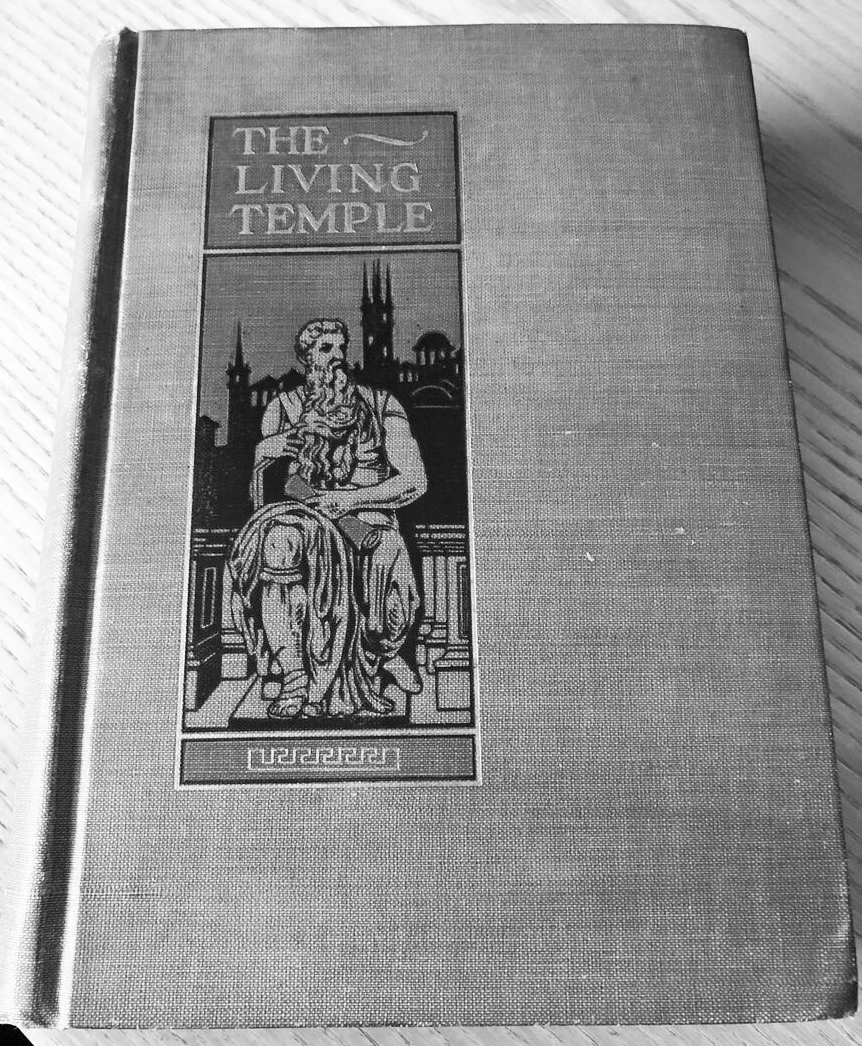
\includegraphics[width=1\linewidth]{images/TLT.jpg}
    \caption*{The Living Temple by Dr. J. H. Kellogg, 1903}
    \label{fig:tlt}
\end{figure}


\begin{figure}[hp]
    \centering
    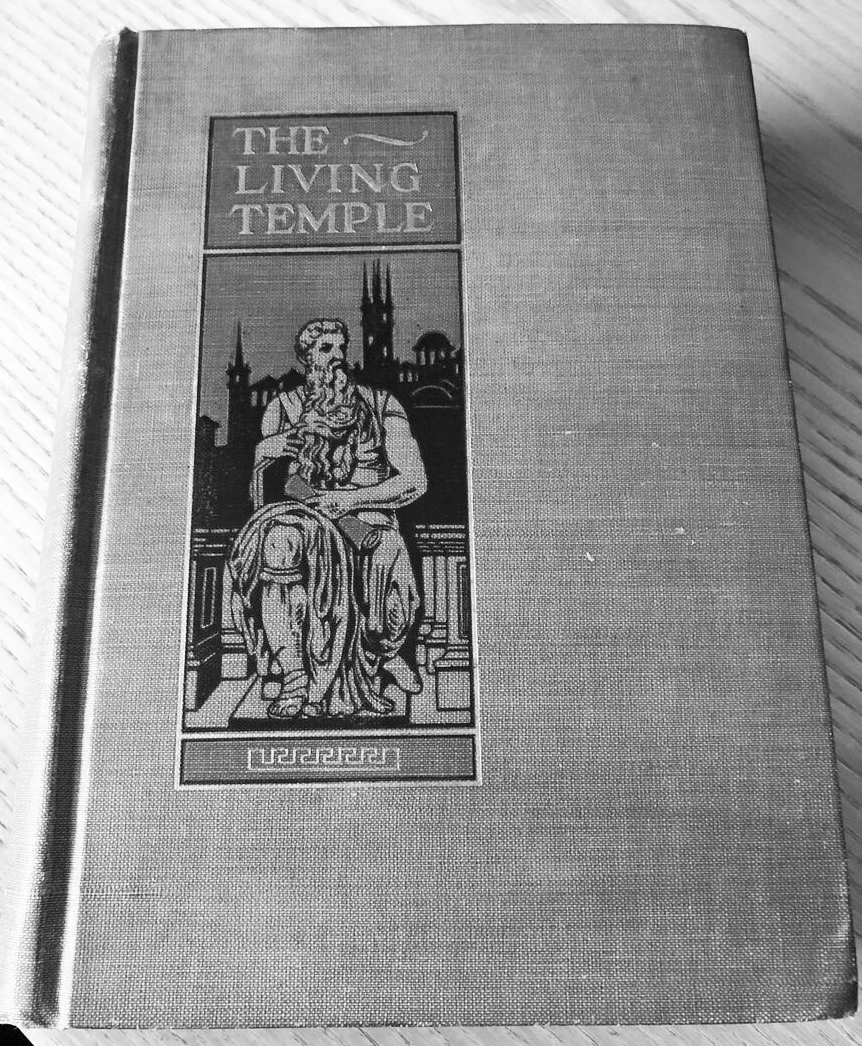
\includegraphics[width=1\linewidth]{images/TLT.jpg}
    \caption*{Le Temple Vivant par Dr. J. H. Kellogg, 1903}
    \label{fig:tlt}
\end{figure}


Some people find Dr. Kellogg’s understanding of God’s personality resonates with their understanding, yet they are tempted to think that there are other things objectionable with the Living Temple. The following evidence suggests the very opposite. There is a letter from Dr. Kellogg to William C. White, where Dr. Kellogg proposes to \others{cutting out a few leaves} from the three thousand copies of the Living Temple—those very leaves containing the \others{specially objectionable things appear, such as the comment on Isaiah 40} and the sentiments regarding the \emcap{personality of God} (the pages we have read).


Certaines personnes trouvent que la compréhension du Dr. Kellogg concernant la personnalité de Dieu résonne avec leur propre compréhension, mais elles sont tentées de penser qu'il y a d'autres choses répréhensibles dans Le Temple Vivant. Les preuves suivantes suggèrent tout le contraire. Il existe une lettre du Dr. Kellogg à William C. White, où le Dr. Kellogg propose de \others{couper quelques pages} des trois mille exemplaires du Temple Vivant—ces mêmes pages contenant les \others{choses particulièrement répréhensibles, comme le commentaire sur Ésaïe 40} et le raisonnement concernant la \emcap{personnalité de Dieu} (les pages que nous avons lues).


\others{The Sanitarium has on hand, I find, \textbf{two or three thousand books which were sold}, but which have come back since the book was condemned. The question has been raised, what shall be done with these? \textbf{It has occurred to me that perhaps they might be saved \underline{by cutting out a few leaves} in which the \underline{specially objectionable things appear}, such as the \underline{comment on Isaiah 40}, which I borrowed from A.T. Jones, and the page on which the unfortunate heading appears, ‘\underline{The Personality of God},’ and tipping in leaves embodying a clear statement of the Bible view of God as a person presented in Elder Haskell’s article in the ‘Review’ a few weeks ago}. These books would be sold to old patients who are making a great demand for the book for Christmas presents…}[Letter from Dr. J.H. Kellogg to W.C.White; December 6, 1903, Chicago][https://174625.selcdn.ru/ellenwhite/EWhite/17226/17226.pdf]


\others{Le Sanatorium a en stock, je trouve, \textbf{deux ou trois mille livres qui ont été vendus}, mais qui sont revenus depuis que le livre a été condamné. La question a été soulevée, que faut-il en faire ? \textbf{Il m'est venu à l'esprit que peut-être ils pourraient être sauvés \underline{en coupant quelques pages} dans lesquelles les \underline{choses particulièrement répréhensibles apparaissent}, comme le \underline{commentaire sur Ésaïe 40}, que j'ai emprunté à A.T. Jones, et la page sur laquelle apparaît le titre malheureux, ‘\underline{La Personnalité de Dieu},’ et en insérant des pages incorporant une déclaration claire de la vision biblique de Dieu en tant que personne présentée dans l'article du Pasteur Haskell dans la ‘Review’ il y a quelques semaines}. Ces livres seraient vendus à d'anciens patients qui font une grande demande pour le livre comme cadeaux de Noël...}[Lettre du Dr. J.H. Kellogg à W.C.White; 6 décembre 1903, Chicago][https://174625.selcdn.ru/ellenwhite/EWhite/17226/17226.pdf]


What is the real issue with the reasoning in the Living Temple? We will study the matter to its very depth; superficially, we clearly see that the issue is the stepping off of the foundation of our faith—the \emcap{Fundamental Principles}—regarding the \emcap{personality of God} and where His presence is.


Quel est le véritable problème avec le raisonnement dans Le Temple Vivant ? Nous étudierons la question en profondeur ; superficiellement, nous voyons clairement que le problème est l'abandon du fondement de notre foi—les \emcap{Principes Fondamentaux}—concernant la \emcap{personnalité de Dieu} et où se trouve Sa présence.


\egw{\textbf{I have been instructed by the heavenly messenger} that \textbf{some of the reasoning} in the book, ‘Living Temple’, is unsound and that \textbf{this reasoning would lead astray} the minds of those who are not thoroughly established on \textbf{the foundation principles} of present truth. \textbf{It introduces that which is naught but speculation} in \textbf{regard to the personality of God and where His presence is}.}[SpTB02 51.3; 1904][https://egwwritings.org/read?panels=p417.262]


\egw{\textbf{J'ai été instruite par le messager céleste} que \textbf{certains des raisonnements} dans le livre ‘Le Temple Vivant’ sont erronés et que \textbf{ce raisonnement égarerait} les esprits de ceux qui ne sont pas fermement établis sur \textbf{les principes fondamentaux} de la vérité présente. \textbf{Il introduit ce qui n'est que spéculation} en \textbf{ce qui concerne la personnalité de Dieu et où est Sa présence}.}[SpTB02 51.3; 1904][https://egwwritings.org/read?panels=p417.262]


Dr. Kellogg introduced the thought \egwinline{which is naught but speculation in regard to the personality of God}, by which he stepped off of the foundation of our faith—the \emcap{Fundamental Principles}. Discordance between Dr. Kellogg’s teaching and the \emcap{Fundamental Principles} is in the first statement of the principles where we are taught that\others{That there is \textbf{one God}, \textbf{a personal, spiritual \underline{being}}, \textbf{the creator of all things}, ... and \textbf{everywhere present by his representative, the Holy Spirit}. Ps. 139:7.}


Le Dr. Kellogg a introduit la pensée \egwinline{qui n'est que spéculation concernant la personnalité de Dieu}, par laquelle il s'est écarté du fondement de notre foi—les \emcap{Principes Fondamentaux}. La discordance entre l'enseignement du Dr. Kellogg et les \emcap{Principes Fondamentaux} se trouve dans la première déclaration des principes où il nous est enseigné qu’\others{Il y a \textbf{un seul Dieu}, \textbf{un \underline{être} personnel et spirituel}, \textbf{le créateur de toutes choses}, ... et \textbf{présent partout par son représentant, le Saint-Esprit}. Ps. 139:7.}


Sister White directly warned us of the sentiments expressed in the Living Temple regarding the \emcap{personality of God}. They are not in harmony with the first point of the \emcap{Fundamental Principles}, which were part of the foundation of our faith.


Sœur White nous a directement mis en garde contre le raisonnement exprimé dans Le Temple Vivant concernant la \emcap{personnalité de Dieu}. Ils ne sont pas en harmonie avec le premier point des \emcap{Principes Fondamentaux}, qui faisaient partie du fondement de notre foi.


\egw{\textbf{I have had to write much concerning the strange doctrines and theories expressed in Living Temple. \underline{Were these theories accepted by our people, the strong pillars of our faith and the truths that have made Seventh-day Adventists what they are would be swept away}. I have had to show the fallacy of these doctrines, presenting them \underline{as a species of last-day heresy}. We are told by the Word of God that just such teaching \underline{will be brought in at this time}.}}[Lt250-1903.2; 1903][https://egwwritings.org/read?panels=p9337.8]


\egw{\textbf{J'ai dû écrire beaucoup concernant les doctrines et théories étranges exprimées dans Le Temple Vivant. \underline{Si ces théories étaient acceptées par notre peuple, les piliers solides de notre foi et les vérités qui ont fait des Adventistes du Septième Jour ce qu'ils sont seraient balayés}. J'ai dû montrer la fausseté de ces doctrines, les présentant \underline{comme une espèce d'hérésie des derniers jours}. La Parole de Dieu nous dit que de tels enseignements \underline{seront introduits en ce temps}.}}[Lt250-1903.2; 1903][https://egwwritings.org/read?panels=p9337.8]


Today we witness the widespread acceptance of Kellogg’s theories regarding the \emcap{personality of God}. The fact that the first point of the \emcap{Fundamental Principles} is no longer present in our beliefs proves that Kellogg’s theories regarding the \emcap{personality of God} have had an influence in shaping our beliefs.


Aujourd'hui, nous assistons à l'acceptation généralisée des théories de Kellogg concernant la \emcap{personnalité de Dieu}. Le fait que le premier point des \emcap{Principes Fondamentaux} ne soit plus présent dans nos croyances prouve que les théories de Kellogg concernant la \emcap{personnalité de Dieu} ont eu une influence dans la formation de nos croyances.


\egw{One and another come to me, asking me to \textbf{explain the positions taken in “Living Temple.”} I reply, “They are unexplainable.” \textbf{The sentiments expressed do not give a true knowledge of God.} \textbf{All through the book are passages of scripture}. \textbf{These scriptures are brought in in such a way \underline{that error is made to appear as truth}}. \textbf{Erroneous theories are presented in so pleasing a way that unless care is taken, many will be misled}.}[SpTB02 52.1; 1904][https://egwwritings.org/read?panels=p417.265]


\egw{L'un après l'autre viennent me voir, me demandant d’\textbf{expliquer les positions prises dans “Le Temple Vivant”.} Je réponds : “Elles sont inexplicables.” \textbf{Le raisonnement exprimé ne donne pas une vraie connaissance de Dieu.} \textbf{Tout au long du livre se trouvent des passages des Écritures}. \textbf{Ces Écritures sont présentées de telle manière \underline{que l'erreur est faite pour apparaître comme la vérité}}. \textbf{Des théories erronées sont présentées d'une manière si plaisante que, sans précaution, beaucoup seront induits en erreur}.}[SpTB02 52.1; 1904][https://egwwritings.org/read?panels=p417.265]


The error is being made to appear as truth, and many are misled.


L'erreur est présentée comme la vérité, et beaucoup sont induits en erreur.


It is worth emphasizing, for some careless reader, that the real issue of Dr. Kellogg, and his book “\textit{Living Temple}”, is not the Trinity but the small step he took off of the \emcap{Fundamental Principles}. In order to understand the real issue of his book, it would be wrong to focus on its overlapping sentiments with the Trinity doctrine. Rather, we should focus on the point that constituted this small step he made; and this includes having a deep understanding of the \emcap{fundamental principles} just as our pioneers had. Who better to ask than the Adventist pioneers themselves?


Il convient de souligner, pour certains lecteurs inattentifs, que le véritable problème du Dr Kellogg et de son livre “\textit{Living Temple}” n'est pas la Trinité, mais le petit pas qu'il a fait en s'écartant des \emcap{Principes Fondamentaux}. Pour comprendre le véritable problème de son livre, il serait erroné de se concentrer sur ses raisonnements qui chevauchent la doctrine de la Trinité. Nous devrions plutôt nous concentrer sur le point qui constituait ce petit pas qu'il a fait; et cela inclut une compréhension profonde des \emcap{principes fondamentaux} tels que nos pionniers les avaient. Qui de mieux à interroger que les pionniers adventistes eux-mêmes?


% Constructive Criticism

\begin{titledpoem}
    
    \stanza{
        A personal God in heaven sits enthroned, \\
        This truth in our Principles firmly zoned. \\
        Present everywhere by Spirit's might, \\
        This foundation stood as our guiding light.
    }

    \stanza{
        Then came words that seemed so wise and deep, \\
        A subtle shift that made the faithful weep. \\
        "God's form beyond all human thought," they claimed, \\
        A mystery too vast to be contained or named.
    }

    \stanza{
        "Discussions of God's form," the Temple said, \\
        "Are futile paths where idols lie ahead." \\
        Yet this philosophy so smoothly spun, \\
        Was the very snare by which souls were won.
    }

    \stanza{
        The error dressed as truth appeared so fair, \\
        As scripture twisted in a clever snare. \\
        One small step from the Principles we held, \\
        One giant leap by which our faith was felled.
    }

    \stanza{
        Beware the mind that thinks itself too wise, \\
        To see deception veiled in truth's disguise. \\
        God is personal, definite, and real, \\
        This is the truth the Temple would conceal. 
    }
\end{titledpoem}